% !TeX TXS-program:compile = txs:///pdflatex/[-shell-escape]
% !TeX TXS-program:pdflatex = pdflatex -synctex=1 -interaction=nonstopmode --shell-escape %.tex
\section{Your First Program}\label{sec:your_first_program}

\sectiontoc

\subsection{Video - Computer Architecture}\label{subsec:video_computer_architecture}

Ok cuando es que se ejecuta un programa, este para que se le pueda pasar a la
computadora, tiene que ser transcrito a lenguaje máquina (binario) y pues bueno
dependiendo de cual es que sea el lenguaje de programación, este va a
ser interpretado o compilado.

\begin{figure}[!ht]
	\centering
	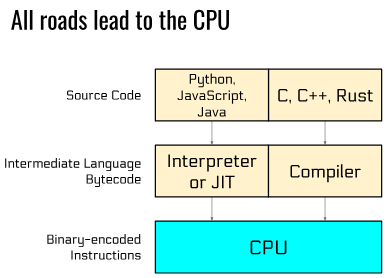
\includegraphics[width=0.8\textwidth]{./img/01_your_first_program/all_roads_lead_to_the_cpu.png}
	\caption{All roads to the CPU}
\end{figure}

Ahora dentro de un CPU, vamos a contar con las compuertas lógicas, siendo
las más comunes la compuerta AND, OR y NOT.

\begin{figure}[!ht]
	\centering
	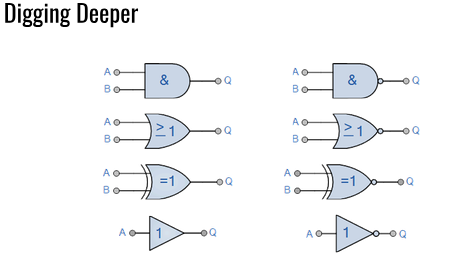
\includegraphics[width=0.8\textwidth]{./img/01_your_first_program/diggin_deeper.png}
	\caption{Digging Deeper}
\end{figure}

\subsection{Video - Assembly}\label{subsec:video_assembly}

Speaking Binary, para nosotros los humanos es complejo el poder hablar
binary code, por eso se creó una representación de texto de dicho
binary code, al cual lo llamamos Assembly.

Luego el video también habla sobre esto de aquí:

\begin{figure}[!ht]
	\centering
	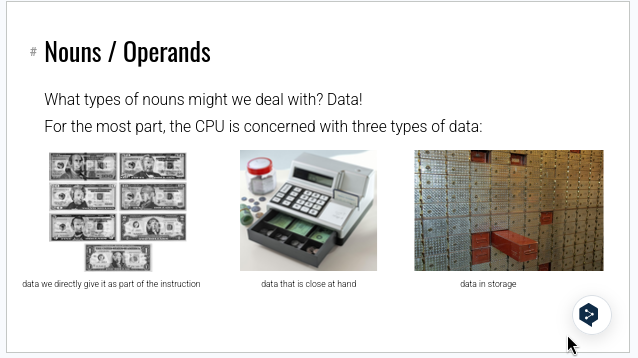
\includegraphics[width=0.8\textwidth]{./img/01_your_first_program/nouns_operands.png}
	\caption{Nouns / Operands}
\end{figure}

\subsection{Video - Registers}\label{subsec:video_registers}

La CPU necesita ser veloz, para esto necesita poder acceder rápidamente a la
información almacenada.

A esto es lo que se le conoce como registros, y contamos con múltiples de ellos
siendo llamados de propósito general, el cual depende de la arquitectura de la
CPU.

\begin{itemize}
	\item Su tamaño suele ser de 64 bits para los computadores modernos.
	\item Podemos acceder de forma parcial a los registros, los primeros 32, 16, 8.
\end{itemize}

\begin{figure}[!ht]
	\centering
	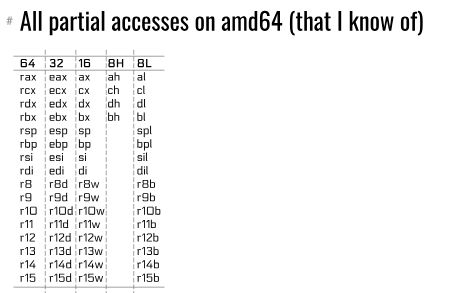
\includegraphics[width=0.8\textwidth]{./img/01_your_first_program/partial_accesses_on_amd64.png}
	\caption{All partial accesses on amd64}
\end{figure}

\begin{figure}[!ht]
	\centering
	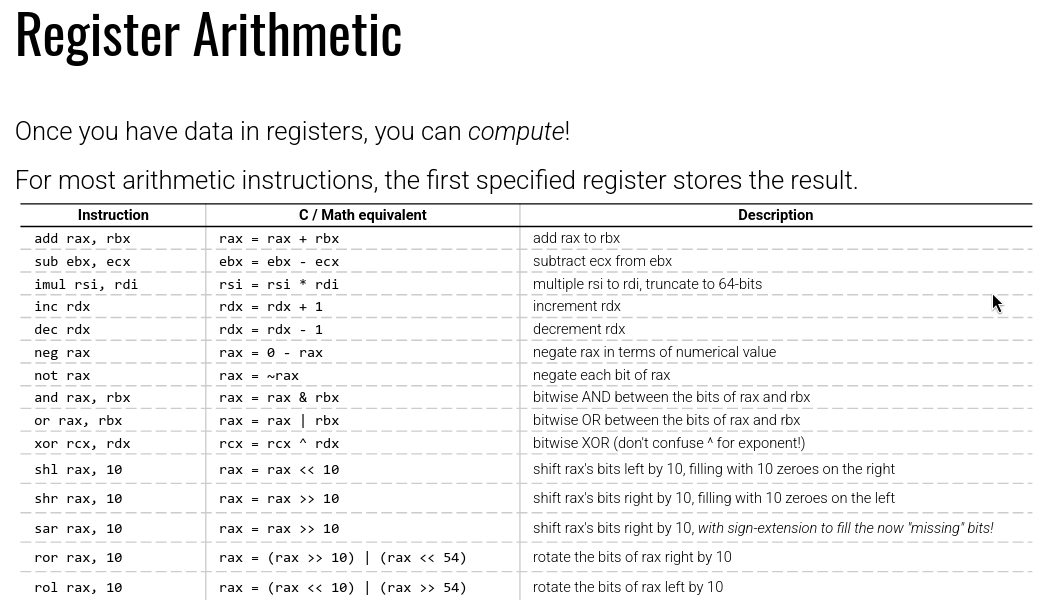
\includegraphics[width=0.8\textwidth]{./img/01_your_first_program/some_instructions.png}
	\caption{Registers Arithmetic}
\end{figure}

Bueno también hace mención que existen otros tipos de registros más "complejos"
o difíciles de trabajar, pero se verá más adelante (creo xD).

\subsection{Your First Register}\label{subsec:your_first_register}

Los registros contienen la data.
La CPU puede poner data en los registros, moverla entre registros y demás.
Así mismo, para el Assembly que se estará trabajando es el x86\_64,
donde contamos con 16 registros de propósito general, como \mintinline{asm}{rax}.

Almacenar un valor a un registro:

\begin{codebox}[ASM]{}
	mov rax, 60
\end{codebox}

\subsection{Your First Syscall}\label{subsec:your_first_syscall}

Los programas interactúan con la CPU usando instrucciones de assembly,
pero para que puedan interactuar con el sistema operativo usan
los \mintinline{asm}{syscall} o \textit{System Call Instruction}.

En Linux contamos alrededor de 330 diferentes \mintinline{asm}{syscall}.

\subsection{Exit Codes}\label{subsec:exit_codes}

Los programas, cuando finalizan, pueden salir con un código de salida al
finalizar.
Este código pasa por el registro \mintinline{asm}{rdx}, el cual indica cuál es dicho
código.

\begin{codebox}[ASM]{}
	mov rdx, 42
	mov rax, 60
	syscall
\end{codebox}

\subsection{Building Executable}\label{subsec:building_executable}

Para compilar un archivo asm (\mintinline{bash}{.S} o \mintinline{bash}{.s}), vamos a usar el comando \mintinline{bash}{as}.
Y para convertirlo en un ejecutable se tiene que usar el comando \mintinline{bash}{ld}.

La directiva \mintinline{asm}{.intel_syntax noprefix}, es usada para indicar que el estilo
de escritura es el de Intel y no queremos usar prefijos especiales para cada
instrucción.

\begin{codebox}[ASM]{}
	.intel_syntax noprefix
	mov rdi, 42
	mov rax, 60
	syscall
\end{codebox}

\subsection{Moving Between Registers}\label{subsec:moving_between_registers}

\begin{codebox}[ASM]{}
	.intel_syntax noprefix
	mov rdi, rsi
	mov rax, 60
	syscall
\end{codebox}
